\section*{4.1 行列式与迹}
\addcontentsline{toc}{section}{4.1 行列式与迹}
\label{sec:4.1}

行列式是线性代数中的重要概念。行列式是线性方程组分析与求解中的一种数学对象。行列式仅对方阵 $ \boldsymbol{A} \in \mathbb{R}^{n \times n} $（即行数与列数相等的矩阵）有定义。在本书中，我们将行列式记为 $ \det(\boldsymbol{A}) $，有时也记作 $ |\boldsymbol{A}| $，因此：

\begin{equation}
\begin{adjustbox}{max width=\linewidth}
\det(\boldsymbol{A}) = \begin{vmatrix} a_{11} & a_{12} & \cdots & a_{1n} \\ a_{21} & a_{22} & \cdots & a_{2n} \\ \vdots & \vdots & \ddots & \vdots \\ a_{n1} & a_{n2} & \cdots & a_{nn} \end{vmatrix}
\end{adjustbox}
\tag{4.1}\label{eq:4-1}
\end{equation}

\emph{备注} 。行列式记号 $ |\boldsymbol{A}| $ 切勿与绝对值混淆。♦

方阵 $ \boldsymbol{A} \in \mathbb{R}^{n \times n} $ 的 \emph{行列式（determinant）} 是一个将 $ \boldsymbol{A} $ 映射到实数的函数。在给出一般 $ n \times n $ 矩阵的行列式定义之前，我们先来看一些具有启发性的示例，并定义一些特殊矩阵的行列式。

\begin{notebox}
\textbf{例 4.1（检验矩阵的可逆性）}
\end{notebox}

\begin{notebox}
我们首先探讨方阵 $ \boldsymbol{A} $ 是否可逆（参见第 2.2.2 节）。对于最小维度的情形，我们已经知道矩阵何时可逆。如果 $ \boldsymbol{A} $ 是 $ 1 \times 1 $ 矩阵（即一个标量），那么 $ \boldsymbol{A} = a \implies \boldsymbol{A}^{-1} = \frac{1}{a} $。因此，$ a \cdot \frac{1}{a} = 1 $ 成立当且仅当 $ a \neq 0 $。
\end{notebox}

\begin{notebox}
对于 $ 2 \times 2 $ 矩阵，由逆矩阵的定义（定义 2.3），我们知道 $ \boldsymbol{A} \boldsymbol{A}^{-1} = \boldsymbol{I} $。结合式~\eqref{eq:2-24}，$ \boldsymbol{A} $ 的逆矩阵为：

\begin{equation}
\boldsymbol{A}^{-1} = \frac{1}{a_{11}a_{22} - a_{12}a_{21}} \begin{bmatrix} a_{22} & -a_{12} \\ -a_{21} & a_{11} \end{bmatrix}
\tag{4.2}\label{eq:4-2}
\end{equation}

因此，$ \boldsymbol{A} $ 可逆当且仅当：

\begin{equation}
a_{11}a_{22} - a_{12}a_{21} \neq 0
\tag{4.3}\label{eq:4-3}
\end{equation}

该量即为 $ \boldsymbol{A} \in \mathbb{R}^{2 \times 2} $ 的行列式，即：

\begin{equation}
\det(\boldsymbol{A}) = \begin{vmatrix} a_{11} & a_{12} \\ a_{21} & a_{22} \end{vmatrix} = a_{11}a_{22} - a_{12}a_{21}
\tag{4.4}\label{eq:4-4}
\end{equation}
\end{notebox}

例 4.1 已经指出了行列式与逆矩阵存在性之间的关系。下面的定理将这一结论推广到一般 $ n \times n $ 矩阵。

\textbf{定理 4.1}。对于任意方阵 $ \boldsymbol{A} \in \mathbb{R}^{n \times n} $，$ \boldsymbol{A} $ 可逆当且仅当 $ \det(\boldsymbol{A}) \neq 0 $。

对于小型矩阵，我们可以根据矩阵元素给出行列式的显式（闭式）表达式。对于 $ n = 1 $：

\begin{equation}
\det(\boldsymbol{A}) = \det(a_{11}) = a_{11}
\tag{4.5}\label{eq:4-5}
\end{equation}

对于 $ n = 2 $：

\begin{equation}
\det(\boldsymbol{A}) = \begin{vmatrix} a_{11} & a_{12} \\ a_{21} & a_{22} \end{vmatrix} = a_{11}a_{22} - a_{12}a_{21}
\tag{4.6}\label{eq:4-6}
\end{equation}

这正是我们在前一个示例中观察到的结果。

对于 $ n = 3 $，对应的计算法则称为 \emph{萨鲁斯法则（Sarrus' rule）} ：

\begin{equation}
\begin{adjustbox}{max width=\linewidth}
\begin{vmatrix} a_{11} & a_{12} & a_{13} \\ a_{21} & a_{22} & a_{23} \\ a_{31} & a_{32} & a_{33} \end{vmatrix} = a_{11}a_{22}a_{33} + a_{21}a_{32}a_{13} + a_{31}a_{12}a_{23} - a_{31}a_{22}a_{13} - a_{11}a_{32}a_{23} - a_{21}a_{12}a_{33}
\end{adjustbox}
\tag{4.7}\label{eq:4-7}
\end{equation}

为了便于记忆萨鲁斯法则中的乘积项，可以尝试在矩阵中画出对角线乘积元素。

如果方阵 $ \boldsymbol{T} $ 满足当 $ i > j $ 时 $ T_{ij} = 0 $（即主对角线下方元素全为 0），我们称其为 \emph{上三角矩阵（upper-triangular matrix）} 。类似地，如果主对角线上方元素全为 0，我们定义其为 \emph{下三角矩阵（lower-triangular matrix）} 。对于三角矩阵 $ \boldsymbol{T} \in \mathbb{R}^{n \times n} $，其行列式是对角线元素的乘积，即：

\begin{equation}
\det(\boldsymbol{T}) = \prod_{i=1}^n T_{ii}
\tag{4.8}\label{eq:4-8}
\end{equation}


\begin{figure}[H]
\centering
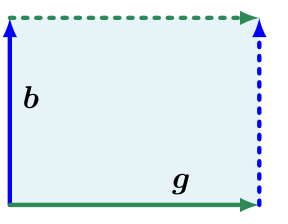
\includegraphics[width=0.92\textwidth,keepaspectratio]{docs/images/Figure4.2.png}
\caption*{\refstepcounter{figcounter}\label{fig:4-2}图~\thefigcounter 由向量 b 和 g 张成的平行四边形（阴影区域）面积为 |det([b, g])|。}
\end{figure}



\begin{figure}[H]
\centering
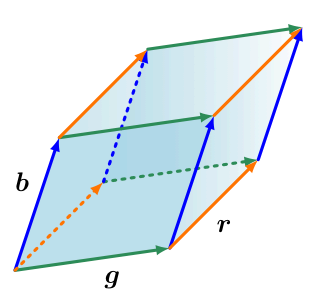
\includegraphics[width=0.92\textwidth,keepaspectratio]{docs/images/Figure4.3.png}
\caption*{\refstepcounter{figcounter}\label{fig:4-3}图~\thefigcounter 由向量 r, b, g 张成的平行六面体（阴影体积）体积为 |det([r, b, g])|。}
\end{figure}


\begin{notebox}
\textbf{例 4.2（行列式作为体积的度量）}
\end{notebox}

\begin{notebox}
当我们将行列式视为从张成 $ \mathbb{R}^n $ 中几何对象的 $ n $ 个向量集合出发的映射时，行列式的概念是非常自然的。事实表明，行列式 $ \det(\boldsymbol{A}) $ 是由矩阵 $ \boldsymbol{A} $ 的列向量构成的 $ n $ 维平行多面体的 \emph{有向体积（signed volume）} 。
\end{notebox}

\begin{notebox}
对于 $ n = 2 $，矩阵的列向量构成一个平行四边形；参见图~\ref{fig:4-2}。随着向量之间的夹角变小，平行四边形的面积也会缩小。考虑构成矩阵 $ \boldsymbol{A} = [\boldsymbol{b}, \boldsymbol{g}] $ 列向量的两个向量 $ \boldsymbol{b}, \boldsymbol{g} $。那么，$ \boldsymbol{A} $ 的行列式绝对值等于以 $ \boldsymbol{0}, \boldsymbol{b}, \boldsymbol{g}, \boldsymbol{b} + \boldsymbol{g} $ 为顶点的平行四边形的面积。特别地，如果 $ \boldsymbol{b}, \boldsymbol{g} $ 线性相关（即对某个 $ \lambda \in \mathbb{R} $ 有 $ \boldsymbol{b} = \lambda \boldsymbol{g} $），它们便不再构成二维平行四边形，因此对应面积为 0。相反，若 $ \boldsymbol{b}, \boldsymbol{g} $ 线性无关且是标准基向量 $ \boldsymbol{e}_1, \boldsymbol{e}_2 $ 的倍数，则它们可以写为

\begin{equation*}
\boldsymbol{b} = \begin{bmatrix} b \\ 0 \end{bmatrix}
\end{equation*}

和

\begin{equation*}
\boldsymbol{g} = \begin{bmatrix} 0 \\ g \end{bmatrix}
\end{equation*}

，行列式为：

\begin{equation*}
\begin{vmatrix} b & 0 \\ 0 & g \end{vmatrix} = bg - 0 = bg
\end{equation*}

行列式的符号表示张成向量 $ \boldsymbol{b}, \boldsymbol{g} $ 相对于标准基 $ (\boldsymbol{e}_1, \boldsymbol{e}_2) $ 的 \emph{定向（orientation）} 。在图~\ref{fig:4-2} 中，若将顺序翻转为 $ \boldsymbol{g}, \boldsymbol{b} $，则交换了 $ \boldsymbol{A} $ 的列，并反转了阴影区域的定向。这就转化为了我们熟悉的公式：$ \textcn{面积} = \textcn{底} \times \textcn{高} $。
\end{notebox}

\begin{notebox}
这种直觉可以推广到更高维度。在 $ \mathbb{R}^3 $ 中，考虑三个向量 $ \boldsymbol{r}, \boldsymbol{b}, \boldsymbol{g} \in \mathbb{R}^3 $ 张成平行六面体的棱，即各个面均为平行四边形的多面体（参见图~\ref{fig:4-3}）。$ 3 \times 3 $ 矩阵 $ [\boldsymbol{r}, \boldsymbol{b}, \boldsymbol{g}] $ 行列式的绝对值就是该立体的体积。因此，行列式充当了度量由矩阵各列向量组合构成的有向体积的函数。
\end{notebox}

\begin{notebox}
考虑如下给出的三个线性无关向量 $ \boldsymbol{r}, \boldsymbol{g}, \boldsymbol{b} \in \mathbb{R}^3 $：

\begin{equation}
\boldsymbol{r} = \begin{bmatrix} 2 \\ 0 \\ -8 \end{bmatrix}, \quad \boldsymbol{g} = \begin{bmatrix} 6 \\ 1 \\ 0 \end{bmatrix}, \quad \boldsymbol{b} = \begin{bmatrix} 1 \\ 4 \\ -1 \end{bmatrix}
\tag{4.9}\label{eq:4-9}
\end{equation}

将这些向量写为矩阵的列：

\begin{equation}
\boldsymbol{A} = [\boldsymbol{r}, \boldsymbol{g}, \boldsymbol{b}] = \begin{bmatrix} 2 & 6 & 1 \\ 0 & 1 & 4 \\ -8 & 0 & -1 \end{bmatrix}
\tag{4.10}\label{eq:4-10}
\end{equation}

这允许我们计算所需的体积：

\begin{equation}
V = |\det(\boldsymbol{A})| = 186
\tag{4.11}\label{eq:4-11}
\end{equation}
\end{notebox}

计算 $ n \times n $ 矩阵的行列式需要一般的算法来求解 $ n > 3 $ 的情形，我们将在下文中进行探讨。下面的定理 4.2 将计算 $ n \times n $ 矩阵行列式的问题归结为计算 $ (n - 1) \times (n - 1) $ 矩阵的行列式。通过递归应用拉普拉斯展开（定理 4.2），我们可以通过最终计算 $ 2 \times 2 $ 矩阵的行列式来计算任意 $ n \times n $ 矩阵的行列式。

\textbf{定理 4.2}（拉普拉斯展开 / Laplace Expansion）。考虑矩阵 $ \boldsymbol{A} \in \mathbb{R}^{n \times n} $。那么对于所有的 $ j = 1, \ldots, n $：

\begin{enumerate}
\item 沿第 $ j $ 列展开：
\end{enumerate}

\begin{equation}
\det(\boldsymbol{A}) = \sum_{k=1}^n (-1)^{k+j} a_{kj} \det(\boldsymbol{A}_{k,j})
\tag{4.12}\label{eq:4-12}
\end{equation}

\begin{enumerate}
\item 沿第 $ j $ 行展开：
\end{enumerate}

\begin{equation}
\det(\boldsymbol{A}) = \sum_{k=1}^n (-1)^{k+j} a_{jk} \det(\boldsymbol{A}_{j,k})
\tag{4.13}\label{eq:4-13}
\end{equation}

这里 $ \boldsymbol{A}_{k,j} \in \mathbb{R}^{(n-1) \times (n-1)} $ 是从 $ \boldsymbol{A} $ 中划去第 $ k $ 行与第 $ j $ 列后得到的子矩阵。$ \det(\boldsymbol{A}_{k,j}) $ 称为 \emph{余子式（minor）} ，而 $ (-1)^{k+j}\det(\boldsymbol{A}_{k,j}) $ 称为 \emph{代数余子式（cofactor）} 。

\begin{notebox}
\textbf{例 4.3（拉普拉斯展开）}
\end{notebox}

\begin{notebox}
我们使用沿第一行的拉普拉斯展开来计算矩阵：

\begin{equation}
\boldsymbol{A} = \begin{bmatrix} 1 & 2 & 3 \\ 3 & 1 & 2 \\ 0 & 0 & 1 \end{bmatrix}
\tag{4.14}\label{eq:4-14}
\end{equation}

的行列式。应用式~\eqref{eq:4-13} 得到：

\begin{equation}
\begin{adjustbox}{max width=\linewidth}
\begin{vmatrix} 1 & 2 & 3 \\ 3 & 1 & 2 \\ 0 & 0 & 1 \end{vmatrix} = (-1)^{1+1} \cdot 1 \begin{vmatrix} 1 & 2 \\ 0 & 1 \end{vmatrix} + (-1)^{1+2} \cdot 2 \begin{vmatrix} 3 & 2 \\ 0 & 1 \end{vmatrix} + (-1)^{1+3} \cdot 3 \begin{vmatrix} 3 & 1 \\ 0 & 0 \end{vmatrix}
\end{adjustbox}
\tag{4.15}\label{eq:4-15}
\end{equation}

利用式~\eqref{eq:4-6} 计算所有 $ 2 \times 2 $ 矩阵的行列式，得到：

\begin{equation}
\det(\boldsymbol{A}) = 1(1 - 0) - 2(3 - 0) + 3(0 - 0) = -5
\tag{4.16}\label{eq:4-16}
\end{equation}

为了完整起见，我们可以将此结果与利用萨鲁斯法则 (4.7) 计算的结果进行比对：

\begin{equation}
\det(\boldsymbol{A}) = 1 \cdot 1 \cdot 1 + 3 \cdot 0 \cdot 3 + 0 \cdot 2 \cdot 2 - 0 \cdot 1 \cdot 3 - 1 \cdot 0 \cdot 2 - 3 \cdot 2 \cdot 1 = 1 - 6 = -5
\tag{4.17}\label{eq:4-17}
\end{equation}
\end{notebox}

对于 $ \boldsymbol{A} \in \mathbb{R}^{n \times n} $，行列式具备以下性质：

\begin{itemize}
\item 矩阵乘积的行列式等于对应行列式的乘积：$ \det(\boldsymbol{A} \boldsymbol{B}) = \det(\boldsymbol{A})\det(\boldsymbol{B}) $。
\item 行列式关于转置不变，即 $ \det(\boldsymbol{A}) = \det(\boldsymbol{A}^\top) $。
\item 若 $ \boldsymbol{A} $ 正则（可逆），则 $ \det(\boldsymbol{A}^{-1}) = \frac{1}{\det(\boldsymbol{A})} $。
\item 相似矩阵（定义 2.22）拥有相同的行列式。因此，对于线性映射 $ \Phi : V \to V $，$ \Phi $ 的所有变换矩阵 $ \boldsymbol{A}_\Phi $ 具有相同的行列式。换言之，行列式与线性映射基的选择无关。
\item 将某一列/行乘上标量后加到另一列/行，不改变 $ \det(\boldsymbol{A}) $。
\item 将某一列/行乘以 $ \lambda \in \mathbb{R} $，使得 $ \det(\boldsymbol{A}) $ 缩放 $ \lambda $ 倍。特别地，$ \det(\lambda \boldsymbol{A}) = \lambda^n \det(\boldsymbol{A}) $。
\item 交换两行/列会改变 $ \det(\boldsymbol{A}) $ 的符号。
\end{itemize}

由于最后三条性质，我们可以使用高斯消元法（参见第 2.1 节）将 $ \boldsymbol{A} $ 化为行阶梯形来计算 $ \det(\boldsymbol{A}) $。当我们将 $ \boldsymbol{A} $ 化为对角线下方全为 0 的三角形式时，便可终止高斯消元。回顾式~\eqref{eq:4-8}，三角矩阵的行列式等于对角线元素的乘积。

\textbf{定理 4.3}。方阵 $ \boldsymbol{A} \in \mathbb{R}^{n \times n} $ 满足 $ \det(\boldsymbol{A}) \neq 0 $ 当且仅当 $ \operatorname{rk}(\boldsymbol{A}) = n $。换言之，$ \boldsymbol{A} $ 可逆当且仅当它是满秩的。

在数学主要依靠手工计算的时代，计算行列式被认为是分析矩阵可逆性的重要途径。然而，现代机器学习方法使用直接数值方法取代了显式行列式计算。例如在第 2 章中，我们学习了逆矩阵可以通过高斯消元法计算。因此，高斯消元法同样可用于计算矩阵的行列式。

行列式在后续章节中具有重要的理论作用，尤其是当我们通过特征多项式学习特征值和特征向量（第 4.2 节）时。

\medskip\hrule\medskip

\section*{4.1.1 迹}
\addcontentsline{toc}{subsection}{4.1.1 迹}

\textbf{定义 4.4}（迹）。方阵 $ \boldsymbol{A} \in \mathbb{R}^{n \times n} $ 的 \emph{迹（trace）} 定义为：

\begin{equation}
\operatorname{tr}(\boldsymbol{A}) := \sum_{i=1}^n a_{ii}
\tag{4.18}\label{eq:4-18}
\end{equation}

即迹是 $ \boldsymbol{A} $ 主对角线上各元素的和。

迹满足以下性质：

\begin{itemize}
\item 对于 $ \boldsymbol{A}, \boldsymbol{B} \in \mathbb{R}^{n \times n} $：$ \operatorname{tr}(\boldsymbol{A} + \boldsymbol{B}) = \operatorname{tr}(\boldsymbol{A}) + \operatorname{tr}(\boldsymbol{B}) $
\item 对于 $ \alpha \in \mathbb{R}, \boldsymbol{A} \in \mathbb{R}^{n \times n} $：$ \operatorname{tr}(\alpha \boldsymbol{A}) = \alpha \operatorname{tr}(\boldsymbol{A}) $
\item $ \operatorname{tr}(\boldsymbol{I}_n) = n $
\item 对于 $ \boldsymbol{A} \in \mathbb{R}^{n \times k}, \boldsymbol{B} \in \mathbb{R}^{k \times n} $：$ \operatorname{tr}(\boldsymbol{A} \boldsymbol{B}) = \operatorname{tr}(\boldsymbol{B} \boldsymbol{A}) $
\end{itemize}

可以证明，同时满足这四个性质的函数是唯一的——即迹函数（Gohberg et al., 2012）。

矩阵乘积的迹具有更一般的性质。特别地，迹在循环排列下保持不变，即：

\begin{equation}
\operatorname{tr}(\boldsymbol{A} \boldsymbol{K} \boldsymbol{L}) = \operatorname{tr}(\boldsymbol{K} \boldsymbol{L} \boldsymbol{A})
\tag{4.19}\label{eq:4-19}
\end{equation}

其中 $ \boldsymbol{A} \in \mathbb{R}^{a \times k}, \boldsymbol{K} \in \mathbb{R}^{k \times l}, \boldsymbol{L} \in \mathbb{R}^{l \times a} $。该性质可推广至任意多个矩阵的乘积。作为式~\eqref{eq:4-19} 的特例，对于两个向量 $ \boldsymbol{x}, \boldsymbol{y} \in \mathbb{R}^n $，有：

\begin{equation}
\operatorname{tr}(\boldsymbol{x} \boldsymbol{y}^\top) = \operatorname{tr}(\boldsymbol{y}^\top \boldsymbol{x}) = \boldsymbol{y}^\top \boldsymbol{x} \in \mathbb{R}
\tag{4.20}\label{eq:4-20}
\end{equation}

给定向量空间 $ V $ 上的线性映射 $ \Phi : V \to V $，我们利用 $ \Phi $ 的矩阵表示的迹来定义该映射的迹。对于 $ V $ 的一组给定基，我们可以通过变换矩阵 $ \boldsymbol{A} $ 描述 $ \Phi $，那么 $ \Phi $ 的迹就是 $ \boldsymbol{A} $ 的迹。对于 $ V $ 的另一组基，对应的变换矩阵 $ \boldsymbol{B} $ 可以通过形如 $ \boldsymbol{S}^{-1}\boldsymbol{A}\boldsymbol{S} $ 的基变换获得（对于某个适当的 $ \boldsymbol{S} $，参见第 2.7.2 节）。对于 $ \Phi $ 对应的迹，这意味着：

\begin{equation}
\operatorname{tr}(\boldsymbol{B}) = \operatorname{tr}(\boldsymbol{S}^{-1}\boldsymbol{A}\boldsymbol{S}) = \operatorname{tr}(\boldsymbol{A}\boldsymbol{S}\boldsymbol{S}^{-1}) = \operatorname{tr}(\boldsymbol{A})
\tag{4.21}\label{eq:4-21}
\end{equation}

因此，尽管线性映射的矩阵表示依赖于基的选择，但线性映射 $ \Phi $ 的迹与基的选择无关。

\medskip\hrule\medskip

\section*{4.1.2 特征多项式}
\addcontentsline{toc}{subsection}{4.1.2 特征多项式}

在本节中，我们介绍了作为刻画方阵函数的行列式与迹。综合我们对行列式与迹的理解，我们现在可以定义一个用多项式描述矩阵 $ \boldsymbol{A} $ 的重要方程，我们将在后续小节中广泛使用它。

\textbf{定义 4.5}（特征多项式）。对于 $ \lambda \in \mathbb{R} $ 和方阵 $ \boldsymbol{A} \in \mathbb{R}^{n \times n} $：

\begin{equation}
p_{\boldsymbol{A}}(\lambda) := \det(\boldsymbol{A} - \lambda \boldsymbol{I})
\tag{4.22a}\label{eq:4-22a}
\end{equation}

\begin{equation}
= c_0 + c_1\lambda + c_2\lambda^2 + \cdots + c_{n-1}\lambda^{n-1} + (-1)^n\lambda^n
\tag{4.22b}\label{eq:4-22b}
\end{equation}

（其中 $ c_0, \ldots, c_{n-1} \in \mathbb{R} $）称为 $ \boldsymbol{A} $ 的 \emph{特征多项式（characteristic polynomial）} 。特别地：

\begin{equation}
c_0 = \det(\boldsymbol{A})
\tag{4.23}\label{eq:4-23}
\end{equation}

\begin{equation}
c_{n-1} = (-1)^{n-1}\operatorname{tr}(\boldsymbol{A})
\tag{4.24}\label{eq:4-24}
\end{equation}

特征多项式~\eqref{eq:4-22a} 将允许我们计算特征值和特征向量，我们将在下一节中进行讨论。
